% arara: xelatex: { shell: yes, synctex: yes }
\documentclass{ist-report}

% == BEGIN PREAMBLE ==
% Packages and configurations here aren't really necessary to define the style,
% but are recommended to use. Some packages require users to know extra commands
% to use properly, so I won't include them in the class file for now.

% -- Code snippets (this one is a challenge to implement)
\usepackage{minted}
\definecolor{bg}{rgb}{0.95,0.95,0.95}
\setminted[c]{linenos, bgcolor = bg, breaklines}
\setmintedinline[c]{bgcolor = {}} 

% -- Bibliography
\usepackage{csquotes}
\usepackage{fvextra}

% -- Extra math options
\usepackage{siunitx}

% -- Extra symbols
\usepackage{amssymb}
\usepackage{textcomp}
\usepackage{gensymb}

% --  Image and float settings
\usepackage{graphicx}
\graphicspath{{graphics/}}
\usepackage{subcaption}

% -- Graphs and diagrams
\usepackage{tikz}
\usepackage{pgfplots}
\usetikzlibrary{arrows.meta,positioning}
\pgfplotsset{compat = 1.5, table/search path = {data/}}
% == END PREAMBLE ==

\newrobustcmd*{\package}[1]{\texttt{#1}}

\begin{document}

\title{Report Example}
\subtitle{Generic implementations of commonly used \LaTeX{} structures}
\author{Daniel de Schiffart}
\date{2018}
\makecover{}

\section{Report Content Samples}

To showcase the class, its effects on multiple \LaTeX{} environments and to give examples on different types of content to use with the class (and with \LaTeX{} in general), this section contains a variety of content to be used within \LaTeX{} and should cover the basis for the content of most reports. Any content not covered here should work fine within this class, as long as there are no conflicting packages, fonts, or other major modifications to the basic \LaTeX{} configuration. Any problems found, report them to me.

\subsection{Basic Math}

This section contains math typesetting as examples to show how it will look like in the final product. This will depend mostly on the font used for math, so the class itself will not have much to change within this department. For the time being, the math font remains imported from the package \package{newpxmath}, which I grew a fondness for. The example from equation \ref{eq:biotsavart} was derived from \textit{The \LaTeX{} Font Catalogue} \cite{fontcatalogue}. It is the integral form of the Biot-Savart law and showcases some details with math font. More math examples to follow.
\begin{gather} \label{eq:biotsavart}
	B(P) = \frac{\mu_0}{4\pi}\int{\frac{\boldsymbol{I} \times \hat{r}'}{r'^2}dl} = \frac{\mu_0}{4\pi} I \int{\frac{d\boldsymbol{l} \times \hat{r}'}{r'^2}}
\end{gather}

An example of arrays and matrices is in equation \ref{eq:sat_error}. The equation in question represents the positioning error $e$ for a group of GPS satellites obtained using differential GPS correction, where $d_{GS}$ represents the distance between satellite $N$ and the differential GPS ground station, and $\rho_{GS}$ the pseudorange obtained in the aforementioned ground station.
\begin{gather} \label{eq:sat_error}
	\left[\begin{matrix}
		e^{(1)} \\
		e^{(2)} \\
		\vdots \\
		e^{(N)} \\
	\end{matrix}\right]
	= \left[\begin{matrix}
		d^{(1)}_{GS} - \rho^{(1)}_{GS} \\
		d^{(2)}_{GS} - \rho^{(2)}_{GS} \\
		\vdots \\
		d^{(N)}_{GS} - \rho^{(N)}_{GS} \\
	\end{matrix}\right]
\end{gather}

\subsection{Floats}

According to the \textit{Wikibooks} \LaTeX{} online textbook \cite{latexwiki},
\begin{quote} \itshape
	Floats are containers for things in a document that cannot be broken over a page. [...] Floats are not part of the normal stream of text, but separate entities, positioned in a part of the page to themselves (top, middle, bottom, left, right, or wherever the designer specifies). They always have a caption describing them and they are always numbered so they can be referred to from elsewhere in the text.
\end{quote}

\subsubsection{Figures}

\begin{figure}[ht]
	\centering
	\includegraphics[width = 0.4\textwidth]{example-image}
	\caption{This is an example image inside a \texttt{figure} float.}
	\label{fig:example}
\end{figure}

\subsubsection{Tables}

My apologies for this section, my \LaTeX{} is kinda shoddy when it comes to tables; I've been kinda making it work with basic \texttt{tabular} environments, like the one in table \ref{tab:ex1}.
\begin{table}[ht]
	\centering
	\begin{tabular}{l c c c}
				& Column 1	& Column 2	& Column 3	\\
	\hline
	Line 1		& $0.0$		& $0.1$		& $0.2$		\\
	Line 2		& $0.4$		& $0.5$		& $0.6$		\\
	Line 3		& $0.8$		& $0.9$		& $1.0$
	\end{tabular}
	\caption{Basic table example.}
	\label{tab:ex1}
\end{table}

\subsection{Ti\textit{k}Z}

A basic Ti\textit{k}Z drawing of a tall box can be found in figure \ref{fig:tikz_ex1}.
\begin{figure}[ht]
	\centering
	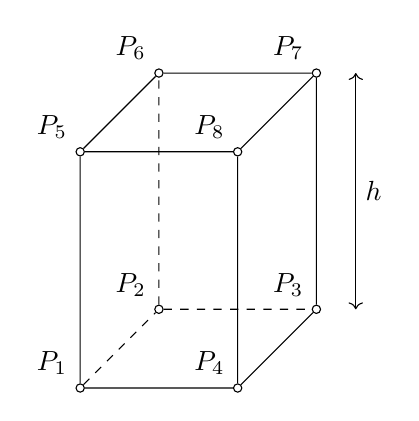
\begin{tikzpicture}[ppoint/.style = {circle,draw,inner sep = 0pt, minimum size = 3pt}]
		\node (p1) at (0,0) [ppoint,label = {135:$P_1$}] {};
		\node (p2) at (1,1) [ppoint,label = {135:$P_2$}] {};
		\node (p3) at (3,1) [ppoint,label = {135:$P_3$}] {};
		\node (p4) at (2,0) [ppoint,label = {135:$P_4$}] {};
		\node (p5) at (0,3) [ppoint,label = {135:$P_5$}] {};
		\node (p6) at (1,4) [ppoint,label = {135:$P_6$}] {};
		\node (p7) at (3,4) [ppoint,label = {135:$P_7$}] {};
		\node (p8) at (2,3) [ppoint,label = {135:$P_8$}] {};
		\draw (p1) -- (p5) -- (p6) -- (p7) -- (p3) -- (p4) -- (p1);
		\draw (p5) -- (p8) -- (p7) (p8) -- (p4);
		\draw [dashed] (p1) -- (p2) -- (p6) (p2) -- (p3);
		\draw [<->] (p3) ++(0.5,0) -- node [auto,swap] {$h$} ++(0,3);
	\end{tikzpicture}
	\caption{Tall box and its corresponding height $h$. Drawing made using Ti\textit{k}Z.}
	\label{fig:tikz_ex1}
\end{figure}

\begin{figure}[ht]
	\centering
	\scalebox{0.8}{
	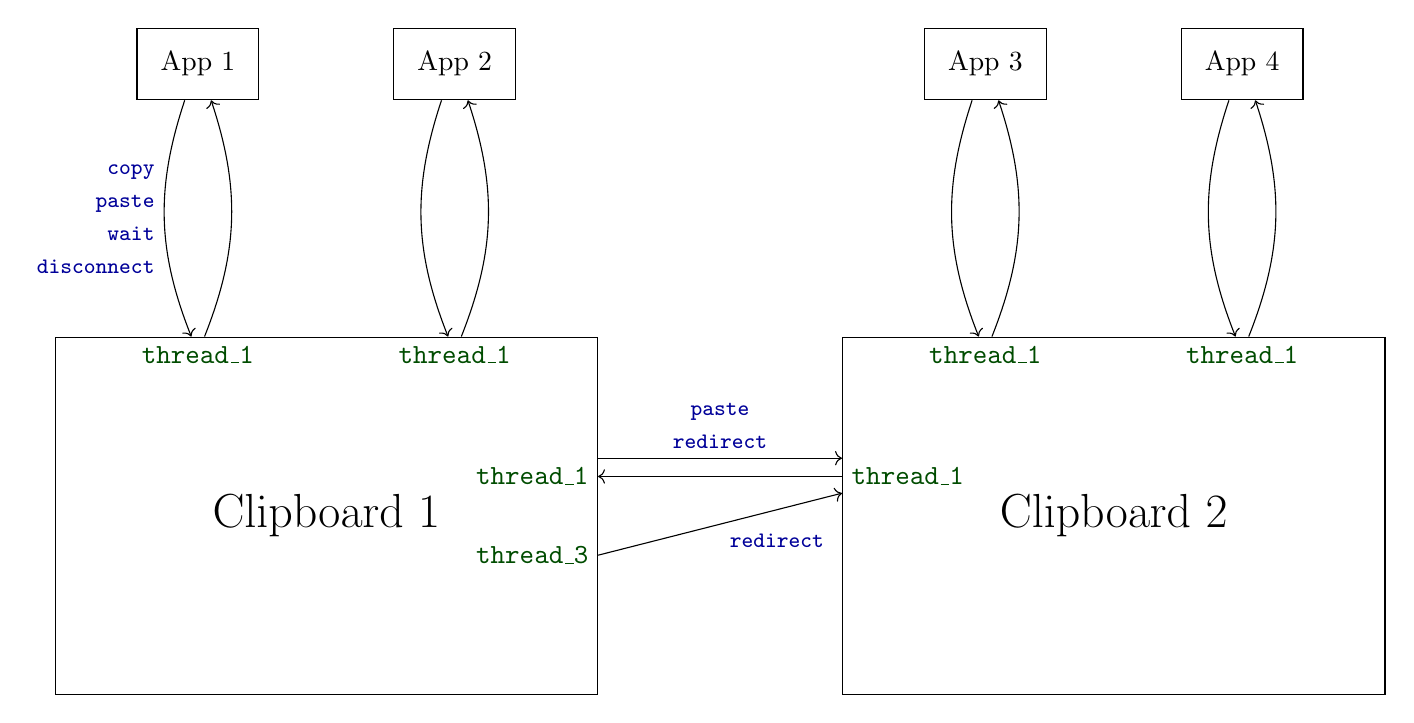
\begin{tikzpicture}[clipboard/.style = {rectangle, draw, inner sep = 2cm},
						app/.style = {rectangle, draw, inner sep = 3mm},
						socketin/.style = {rectangle, color = black!70!green},
						pathstyle/.style = {->},
						pathlabel/.style ={color = black!40!blue}]
		% Start of Clipboard 1
		\node (app1) at (0,0) [app] {App 1};
		\node (app2) [app, right = 1.7cm of app1] {App 2};
		\node (t2app1) [socketin, below = 3cm of app1] {\texttt{thread\_1}};
		\node (t2app2) [socketin, below = 3cm of app2] {\texttt{thread\_1}};
		\draw [pathstyle] (app1) to [bend right = 20] node [auto,swap,align = right, pathlabel] {\footnotesize \ttfamily copy \\ \footnotesize \ttfamily paste \\ \footnotesize \ttfamily wait \\ \footnotesize \ttfamily disconnect} (t2app1);
		\draw [pathstyle] (t2app1) to [bend right = 20] (app1);
		\draw [pathstyle] (app2) to [bend right = 20] (t2app2);
		\draw [pathstyle] (t2app2) to [bend right = 20] (app2);
		\path (t2app1.north) to node (clip1) [auto, swap, clipboard] {\LARGE Clipboard 1} (t2app2.north);
		\path (clip1.north east) to node (clip1in1) [auto, swap, align = right, yshift = 0.5cm, socketin] {\texttt{thread\_1}} node (clip1in3) [auto, swap, align = right, yshift = -0.5cm, socketin] {\texttt{thread\_3}} (clip1.south east);
		% Start of Clipboard 2
		\node (app3) at (10,0) [app] {App 3};
		\node (app4) [app, right = 1.7cm of app3] {App 4};
		\node (t2app3) [socketin, below = 3cm of app3] {\texttt{thread\_1}};
		\node (t2app4) [socketin, below = 3cm of app4] {\texttt{thread\_1}};
		\draw [pathstyle] (app3) to [bend right = 20] (t2app3);
		\draw [pathstyle] (t2app3) to [bend right = 20] (app3);
		\draw [pathstyle] (app4) to [bend right = 20] (t2app4);
		\draw [pathstyle] (t2app4) to [bend right = 20] (app4);
		\path (t2app3.north) to node (clip2) [auto, swap, clipboard] {\LARGE Clipboard 2} (t2app4.north);
		\path (clip2.north west) to node (clip2in1) [auto, align = left, yshift = 0.5cm, socketin] {\texttt{thread\_1}} (clip2.south west);
		% Paths in between
		\draw [pathstyle] (clip1in1.north east) -- node [auto, align = center, pathlabel] {\ttfamily \footnotesize paste \\ \ttfamily \footnotesize redirect} (clip2in1.north west);
		\draw [pathstyle] (clip2in1) -- (clip1in1);
		\draw [pathstyle] (clip1in3.east) -- node [auto, swap, pathlabel] {\ttfamily \footnotesize redirect} (clip2in1);
	\end{tikzpicture}}
	\caption{A slightly longer T\textit{i}kZ example.}
	\label{fig:scheme_main}
\end{figure}

\subsection{Plots}

\subsection{Code Snippets and Extracts}

The objective is to have any code content use the \package{minted} package to typeset code. However, due to the high number of requirements to properly run \package{minted} on a local installation of \TeX{}, this option should only be used with an online editor (\textit{Overleaf} comes as the most prominent example). In any case, for the time being \package{minted} is included in this template, but can be further on replaced with a package like \package{listings}, possibly using a class option. Plans are also down to include a tutorial on how to check and install \package{minted} and get it to work.

Here is a basic excerpt of a basic C \textit{Hello World} program.
\begin{minted}{c}
#include <stdio.h>

int main(void)
{
    printf("Hello World!");
    
    return 0;
}
\end{minted}

\end{document}
